\documentclass[11pt,a4paper]{article}
\usepackage{amsmath,amssymb,graphicx,enumitem,tikz,xcolor,needspace}
\usetikzlibrary{calc}
\usepackage[margin=2.2cm]{geometry}
\setlength{\parindent}{0pt}
\setlength{\parskip}{5pt}
\renewcommand{\arraystretch}{1.2}

% Layout helper for the textbook figures (Fig. 7.6 and Fig. 7.8): a 10 x 10 grid
% with columns labelled along the bottom and rows labelled up the side.
% Only the points passed in the argument are drawn; no coordinates are printed.
\newcommand{\ncertgrid}[1]{%
\begin{tikzpicture}[scale=0.5]
\fill[cyan!12] (0,0) rectangle (10,10);
\draw[step=1,gray!60,very thin] (0,0) grid (10,10);
\draw[thick] (0,0) rectangle (10,10);
\foreach \i in {0,...,10}{\node[below,font=\scriptsize] at (\i,0) {\i};}
\foreach \i in {1,...,10}{\node[left,font=\scriptsize] at (0,\i) {\i};}
\node[below,font=\small\bfseries] at (5,-0.8) {Columns};
\node[rotate=90,above,font=\small\bfseries] at (-1.0,5) {Rows};
#1
\end{tikzpicture}}


% never leave a question heading stranded at the foot of a page
\let\oldsubsection\subsection
\renewcommand{\subsection}{\Needspace{12\baselineskip}\oldsubsection}

% ---- final result of a solution, highlighted inside the Solution (not a separate section) ----
\newcommand{\figcap}[1]{\\*[-2pt]{\small #1}}
\newcommand{\ans}[1]{\par\vspace{4pt}\noindent\fcolorbox{black!55}{blue!6}{\parbox{\dimexpr\linewidth-2\fboxsep-2\fboxrule\relax}{\raggedright\textbf{Answer:} #1}}\par\vspace{2pt}}

% ---- common mistake note for students who got this step wrong ----
\newcommand{\slip}[1]{\par\noindent{\small\itshape\textbf{Common mistake.} #1}\par}

% ---- distance formula written out in full, so every value can be checked ----
% \bk{n}      : n, in brackets when n is negative
% \dist{AB}{x1}{y1}{x2}{y2}{simplified value}   rows of an align* (add a line break after it)
% \distn{AB}{x1}{y1}{x2}{y2}                      same, when the root does not simplify
% Rows: (1) substitute into the formula, (2) work out each difference,
%       (3) square each difference, (4) add the squares, then take the root.
\newcommand{\bk}[1]{\ifnum#1<0 (#1)\else #1\fi}
\newcommand{\distcore}[5]{#1&=\sqrt{(#4-\bk{#2})^2+(#5-\bk{#3})^2}\\
&=\sqrt{\bk{\the\numexpr#4-#2\relax}^2+\bk{\the\numexpr#5-#3\relax}^2}\\
&=\sqrt{\the\numexpr(#4-#2)*(#4-#2)\relax+\the\numexpr(#5-#3)*(#5-#3)\relax}
=\sqrt{\the\numexpr(#4-#2)*(#4-#2)+(#5-#3)*(#5-#3)\relax}}
\newcommand{\distnote}{\textit{How to read the working below:} in each pair the first point named is $(x_1,y_1)$ and the second is $(x_2,y_2)$. Line 1 puts the values into the formula, line 2 works out each bracket, line 3 squares the brackets, and then the squares are added and the square root is taken.}
\newcommand{\dist}[6]{\distcore{#1}{#2}{#3}{#4}{#5}=#6}
\newcommand{\distn}[5]{\distcore{#1}{#2}{#3}{#4}{#5}}

\begin{document}

\begin{center}
{\Large\bfseries Class 10 Mathematics (NCERT) -- Chapter 7: Coordinate Geometry}\\[4pt]
{\large Worked solutions: Examples 1--10, Exercise 7.1 and Exercise 7.2}\\[2pt]
{\small Reprint 2026--27 edition. Draft for teacher verification.}
\end{center}

\subsection*{Formulas used in this chapter}
\begin{enumerate}[label=(F\arabic*),leftmargin=*]
\item \textbf{Distance formula.} The distance between $P(x_1,y_1)$ and $Q(x_2,y_2)$ is
\[PQ=\sqrt{(x_2-x_1)^2+(y_2-y_1)^2}.\]
\item \textbf{Distance from the origin.} $OP=\sqrt{x^2+y^2}$ for $P(x,y)$.
\item \textbf{Section formula (internal division).} The point $P$ dividing the segment joining $A(x_1,y_1)$ and $B(x_2,y_2)$ internally in the ratio $m_1:m_2$ is
$P\left(\dfrac{m_1x_2+m_2x_1}{m_1+m_2},\ \dfrac{m_1y_2+m_2y_1}{m_1+m_2}\right)$.
\item \textbf{Mid-point formula.} The mid-point of $A(x_1,y_1)$ and $B(x_2,y_2)$ is $\left(\dfrac{x_1+x_2}{2},\dfrac{y_1+y_2}{2}\right)$ (section formula with $m_1:m_2=1:1$).
\item A point on the $x$-axis has the form $(x,0)$ and a point on the $y$-axis has the form $(0,y)$.
\end{enumerate}

\section*{Part A: Solved Examples 1 to 5 (Section 7.2, Distance Formula)}

%---------------------------------------------------------------
\subsection*{Example 1}
\textbf{Question.} Do the points $(3,2)$, $(-2,-3)$ and $(2,3)$ form a triangle? If so, name the type of triangle formed.

\textbf{Solution.} Let $P(3,2)$, $Q(-2,-3)$ and $R(2,3)$.

\textbf{Step 1: find the three sides.} By the distance formula, the distance between $(x_1,y_1)$ and $(x_2,y_2)$ is
\[d=\sqrt{(x_2-x_1)^2+(y_2-y_1)^2}.\]
\distnote
\begin{align*}
\dist{PQ}{3}{2}{-2}{-3}{5\sqrt2\approx 7.07}\\
\dist{QR}{-2}{-3}{2}{3}{2\sqrt{13}\approx 7.21}\\
\distn{PR}{3}{2}{2}{3}\approx 1.41
\end{align*}
\slip{A negative number squared is positive: $(-5)^2=25$, not $-25$. Also $-2-3=-5$ (not $1$), and $2-(-2)=2+2=4$.}

\textbf{Step 2: do the points form a triangle?} Three points form a triangle only if the sum of any two of the distances is greater than the third. Using the values above ($PQ\approx7.07$, $QR\approx7.21$, $PR\approx1.41$):
\begin{align*}
PQ+PR&\approx 7.07+1.41=8.48>QR\ (\approx7.21)\\
QR+PR&\approx 7.21+1.41=8.62>PQ\ (\approx7.07)\\
PQ+QR&\approx 7.07+7.21=14.28>PR\ (\approx1.41)
\end{align*}
All three hold, so $P,Q,R$ are not in a straight line and form a triangle.

\textbf{Step 3: what type of triangle?} By the converse of the Pythagoras theorem (if $a^2+b^2=c^2$ for the sides of a triangle, the angle opposite $c$ is $90^\circ$). The square of each side is the number under its square root in Step 1: $PQ^2=50$, $PR^2=2$, $QR^2=52$. The longest side is $QR$, so test it:
\[
PQ^2+PR^2=50+2=52=QR^2 .
\]
So the angle opposite $QR$, which is $\angle P$, is $90^\circ$. The sides $PQ,QR,PR$ are all different, so the triangle is not isosceles; it is a right-angled triangle.

\ans{The points form a triangle. It is a right-angled triangle, with the right angle at $P$.}

%---------------------------------------------------------------
\subsection*{Example 2}
\textbf{Question.} Show that the points $(1,7)$, $(4,2)$, $(-1,-1)$ and $(-4,4)$ are the vertices of a square.

\textbf{Solution.} Let $A(1,7)$, $B(4,2)$, $C(-1,-1)$, $D(-4,4)$.

A quadrilateral is a square if all four sides are equal and both diagonals are equal. By the distance formula $d=\sqrt{(x_2-x_1)^2+(y_2-y_1)^2}$, find the four sides and the two diagonals.

\distnote
\begin{align*}
\distn{AB}{1}{7}{4}{2}\\
\distn{BC}{4}{2}{-1}{-1}\\
\distn{CD}{-1}{-1}{-4}{4}\\
\distn{DA}{-4}{4}{1}{7}\\
\dist{AC}{1}{7}{-1}{-1}{2\sqrt{17}}\\
\dist{BD}{4}{2}{-4}{4}{2\sqrt{17}}
\end{align*}
Here $\sqrt{34}$ cannot be simplified, and $\sqrt{68}=\sqrt{4\times17}=2\sqrt{17}$.

Since $AB=BC=CD=DA=\sqrt{34}$ and $AC=BD=2\sqrt{17}$, all four sides are equal and the two diagonals are equal.

\ans{$ABCD$ is a square.}

\textbf{Alternative solution.} Using the converse of the Pythagoras theorem in $\triangle ADC$: $AD^2+DC^2=34+34=68=AC^2$ (the values $34$, $34$, $68$ are the numbers under the square roots above), so $\angle D=90^\circ$. A quadrilateral with all four sides equal and one angle $90^\circ$ is a square.

%---------------------------------------------------------------
\subsection*{Example 3}
\textbf{Question.} Fig.\ 7.6 shows the arrangement of desks in a classroom. Ashima, Bharti and Camella are seated at $A(3,1)$, $B(6,4)$ and $C(8,6)$ respectively. Do you think they are seated in a line? Give reasons for your answer.

\begin{center}
\ncertgrid{\fill (3,1) circle (3pt) node[above left]{$A$};
\fill (6,4) circle (3pt) node[above left]{$B$};
\fill (8,6) circle (3pt) node[above left]{$C$};}\\
{\small Fig.\ 7.6 (redrawn)}
\end{center}

\textbf{Solution.} The coordinates of the seats are given in the question: $A(3,1)$, $B(6,4)$, $C(8,6)$.

Three points are collinear if the largest of the three distances equals the sum of the other two. By the distance formula $d=\sqrt{(x_2-x_1)^2+(y_2-y_1)^2}$:

\distnote
\begin{align*}
\dist{AB}{3}{1}{6}{4}{3\sqrt2}\\
\dist{BC}{6}{4}{8}{6}{2\sqrt2}\\
\dist{AC}{3}{1}{8}{6}{5\sqrt2}
\end{align*}
Here $\sqrt{18}=\sqrt{9\times2}=3\sqrt2$, $\sqrt8=\sqrt{4\times2}=2\sqrt2$ and $\sqrt{50}=\sqrt{25\times2}=5\sqrt2$.

The largest distance is $AC=5\sqrt2$. Add the other two:
\[
AB+BC=3\sqrt2+2\sqrt2=(3+2)\sqrt2=5\sqrt2=AC .
\]
\ans{Since $AB+BC=AC$, the points $A$, $B$, $C$ are collinear. Ashima, Bharti and Camella are seated in a line.}

%---------------------------------------------------------------
\subsection*{Example 4}
\textbf{Question.} Find a relation between $x$ and $y$ such that the point $(x,y)$ is equidistant from the points $(7,1)$ and $(3,5)$.

\textbf{Solution.} Let $P(x,y)$ be equidistant from $A(7,1)$ and $B(3,5)$, so $AP=BP$ and therefore $AP^2=BP^2$ (squaring removes the square roots).

By the distance formula, $d^2=(x_2-x_1)^2+(y_2-y_1)^2$, so
\[
AP^2=(x-7)^2+(y-1)^2,\qquad BP^2=(x-3)^2+(y-5)^2 .
\]
Equate them and expand each bracket with $(a-b)^2=a^2-2ab+b^2$:
\begin{align*}
(x-7)^2+(y-1)^2&=(x-3)^2+(y-5)^2\\
(x^2-14x+49)+(y^2-2y+1)&=(x^2-6x+9)+(y^2-10y+25)\\
x^2+y^2-14x-2y+50&=x^2+y^2-6x-10y+34
\end{align*}
Cancel $x^2+y^2$ from both sides and collect the terms on the left:
\begin{align*}
-14x-2y+50&=-6x-10y+34\\
-14x+6x-2y+10y+50-34&=0\\
-8x+8y+16&=0\\
x-y&=2\qquad(\text{dividing by }-8)
\end{align*}
\slip{When expanding $(x-7)^2$ the middle term $-14x$ is often forgotten; $(x-7)^2\neq x^2-49$.}

\textbf{Verification.} The point $(4,2)$ satisfies $x-y=4-2=2$. Its distances from $A(7,1)$ and $B(3,5)$ are
\begin{align*}
\distn{AP}{7}{1}{4}{2}\\
\distn{BP}{3}{5}{4}{2}
\end{align*}
Both are $\sqrt{10}$, so the point is equidistant, as required.

\ans{The required relation is $x-y=2$.}

%---------------------------------------------------------------
\subsection*{Example 5}
\textbf{Question.} Find a point on the $y$-axis which is equidistant from the points $A(6,5)$ and $B(-4,3)$.

\textbf{Solution.} A point on the $y$-axis has the form $(0,y)$ (its $x$-coordinate is $0$). Let $P(0,y)$ be equidistant from $A$ and $B$, so $PA=PB$ and $PA^2=PB^2$.

By the distance formula $d^2=(x_2-x_1)^2+(y_2-y_1)^2$:
\[
PA^2=(6-0)^2+(5-y)^2,\qquad PB^2=(-4-0)^2+(3-y)^2 .
\]
Equate them and expand with $(a-b)^2=a^2-2ab+b^2$:
\begin{align*}
(6-0)^2+(5-y)^2&=(-4-0)^2+(3-y)^2\\
36+(25-10y+y^2)&=16+(9-6y+y^2)\\
61-10y+y^2&=25-6y+y^2\\
61-10y&=25-6y\\
36&=4y\\
y&=9
\end{align*}
So $P=(0,9)$.

\textbf{Verification.} With $P(0,9)$:
\begin{align*}
\dist{PA}{0}{9}{6}{5}{2\sqrt{13}}\\
\dist{PB}{0}{9}{-4}{3}{2\sqrt{13}}
\end{align*}
Both distances are $\sqrt{52}=2\sqrt{13}$.

\ans{The required point is $(0,9)$.}

\newpage
\section*{Part B: Exercise 7.1}

%---------------------------------------------------------------
\subsection*{Exercise 7.1, Question 1}
\textbf{Question.} Find the distance between the following pairs of points:\\
(i) $(2,3),\ (4,1)$\\
(ii) $(-5,7),\ (-1,3)$\\
(iii) $(a,b),\ (-a,-b)$

\textbf{Solution.} By the distance formula, the distance between $P(x_1,y_1)$ and $Q(x_2,y_2)$ is
\[PQ=\sqrt{(x_2-x_1)^2+(y_2-y_1)^2}.\]
\distnote

\textbf{(i)} $(x_1,y_1)=(2,3)$ and $(x_2,y_2)=(4,1)$:
\begin{align*}
\dist{d}{2}{3}{4}{1}{2\sqrt2}
\end{align*}
Here $\sqrt8=\sqrt{4\times2}=2\sqrt2$.

\textbf{(ii)} $(x_1,y_1)=(-5,7)$ and $(x_2,y_2)=(-1,3)$:
\begin{align*}
\dist{d}{-5}{7}{-1}{3}{4\sqrt2}
\end{align*}
Here $\sqrt{32}=\sqrt{16\times2}=4\sqrt2$.

\textbf{(iii)} $(x_1,y_1)=(a,b)$ and $(x_2,y_2)=(-a,-b)$:
\begin{align*}
d&=\sqrt{(-a-a)^2+(-b-b)^2}\\
&=\sqrt{(-2a)^2+(-2b)^2}\\
&=\sqrt{4a^2+4b^2}=\sqrt{4(a^2+b^2)}=2\sqrt{a^2+b^2}
\end{align*}
\slip{$\sqrt{4a^2+4b^2}$ is not $2a+2b$: the square root of a sum is not the sum of the square roots. Factor out $4$ first.}

\textbf{Verification.} For (iii) take $a=3$, $b=4$. The points are $(3,4)$ and $(-3,-4)$:
\[
\sqrt{(-3-3)^2+(-4-4)^2}=\sqrt{(-6)^2+(-8)^2}=\sqrt{36+64}=\sqrt{100}=10,
\]
and the formula gives $2\sqrt{3^2+4^2}=2\sqrt{25}=2\times5=10$. The two agree.

\ans{(i) $2\sqrt2$ units; (ii) $4\sqrt2$ units; (iii) $2\sqrt{a^2+b^2}$ units.}

%---------------------------------------------------------------
\subsection*{Exercise 7.1, Question 2}
\textbf{Question.} Find the distance between the points $(0,0)$ and $(36,15)$. Can you now find the distance between the two towns $A$ and $B$ discussed in Section 7.2.

(Section 7.2: A town $B$ is located 36 km east and 15 km north of the town $A$.)

\textbf{Solution.} By the distance formula, $d=\sqrt{(x_2-x_1)^2+(y_2-y_1)^2}$, with $(x_1,y_1)=(0,0)$ and $(x_2,y_2)=(36,15)$:
\begin{align*}
\dist{d}{0}{0}{36}{15}{39}
\end{align*}
Here $36^2=1296$, $15^2=225$, $1296+225=1521$ and $39^2=1521$, so $\sqrt{1521}=39$.

Now the towns. Take town $A$ as the origin $(0,0)$, one unit as 1~km, east as the positive $x$-direction and north as the positive $y$-direction. Then town $B$, 36 km east and 15 km north of $A$, is at $(36,15)$. So the distance between the towns is the distance between $(0,0)$ and $(36,15)$.

\ans{The distance between $(0,0)$ and $(36,15)$ is $39$ units. Yes, the distance between the towns $A$ and $B$ is $39$ km.}

%---------------------------------------------------------------
\subsection*{Exercise 7.1, Question 3}
\textbf{Question.} Determine if the points $(1,5)$, $(2,3)$ and $(-2,-11)$ are collinear.

\textbf{Solution.} Let $A(1,5)$, $B(2,3)$, $C(-2,-11)$.

Three points are collinear if the largest of the three distances equals the sum of the other two. By the distance formula $d=\sqrt{(x_2-x_1)^2+(y_2-y_1)^2}$:

\distnote
\begin{align*}
\distn{AB}{1}{5}{2}{3}\approx2.24\\
\dist{BC}{2}{3}{-2}{-11}{2\sqrt{53}\approx14.56}\\
\distn{AC}{1}{5}{-2}{-11}\approx16.28
\end{align*}
Here $\sqrt{212}=\sqrt{4\times53}=2\sqrt{53}$.

The largest distance is $AC\approx16.28$. The sum of the other two is
\[AB+BC\approx2.24+14.56=16.80\neq16.28\approx AC.\]
For an exact check, suppose $\sqrt5+\sqrt{212}=\sqrt{265}$. Squaring both sides, with $(p+q)^2=p^2+2pq+q^2$:
\[5+212+2\sqrt{5\times212}=265\ \Rightarrow\ 2\sqrt{1060}=48\ \Rightarrow\ \sqrt{1060}=24\ \Rightarrow\ 1060=24^2=576,\]
which is false. So $AB+BC\neq AC$.
\slip{Compare the largest distance with the sum of the \emph{other two}. Comparing $AB+AC$ with $BC$ proves nothing.}

\textbf{Alternative solution (section formula).} If $C$ lay on line $AB$, it would divide $AB$ in some ratio $k:1$, and by the section formula $\left(\dfrac{m_1x_2+m_2x_1}{m_1+m_2},\dfrac{m_1y_2+m_2y_1}{m_1+m_2}\right)$ with $A(1,5)$, $B(2,3)$, $m_1:m_2=k:1$,
\[C=\left(\frac{k(2)+1(1)}{k+1},\frac{k(3)+1(5)}{k+1}\right)=\left(\frac{2k+1}{k+1},\frac{3k+5}{k+1}\right).\]
From the $x$-coordinate: $\dfrac{2k+1}{k+1}=-2\Rightarrow 2k+1=-2k-2\Rightarrow k=-\dfrac34$.\\
From the $y$-coordinate: $\dfrac{3k+5}{k+1}=-11\Rightarrow 3k+5=-11k-11\Rightarrow k=-\dfrac87$.\\
The two values of $k$ differ, so no single ratio puts $C$ on line $AB$.

\ans{The points are not collinear.}

%---------------------------------------------------------------
\subsection*{Exercise 7.1, Question 4}
\textbf{Question.} Check whether $(5,-2)$, $(6,4)$ and $(7,-2)$ are the vertices of an isosceles triangle.

\textbf{Solution.} Let $A(5,-2)$, $B(6,4)$, $C(7,-2)$.

By the distance formula $d=\sqrt{(x_2-x_1)^2+(y_2-y_1)^2}$:

\distnote
\begin{align*}
\distn{AB}{5}{-2}{6}{4}\\
\distn{BC}{6}{4}{7}{-2}\\
\dist{AC}{5}{-2}{7}{-2}{2}
\end{align*}
(Here $\sqrt{37}\approx6.08$, and $\sqrt4=2$.)

\textbf{Do the points form a triangle?} They do if the sum of any two distances is greater than the third:
\begin{align*}
AB+BC&\approx6.08+6.08=12.16>AC=2\\
AB+AC&\approx6.08+2=8.08>BC\approx6.08\\
BC+AC&\approx6.08+2=8.08>AB\approx6.08
\end{align*}
\textbf{Is it isosceles?} A triangle is isosceles if two of its sides are equal. Here $AB=BC=\sqrt{37}$.

\ans{Yes, the points are the vertices of an isosceles triangle, with $AB=BC=\sqrt{37}$ units.}

%---------------------------------------------------------------
\subsection*{Exercise 7.1, Question 5}
\textbf{Question.} In a classroom, 4 friends are seated at the points $A$, $B$, $C$ and $D$ as shown in Fig.\ 7.8. Champa and Chameli walk into the class and after observing for a few minutes Champa asks Chameli, ``Don't you think $ABCD$ is a square?'' Chameli disagrees. Using distance formula, find which of them is correct.

\begin{center}
\ncertgrid{\fill (3,4) circle (3pt) node[above left]{$A$};
\fill (6,7) circle (3pt) node[above left]{$B$};
\fill (9,4) circle (3pt) node[above right]{$C$};
\fill (6,1) circle (3pt) node[above left]{$D$};}\\
{\small Fig.\ 7.8 (redrawn)}
\end{center}

\textbf{Solution.} \emph{Reading the figure.} In Fig.\ 7.8 the horizontal axis is labelled Columns and the vertical axis is labelled Rows. We take the column number as the $x$-coordinate and the row number as the $y$-coordinate. From the figure:
$A$ is in column 3, row 4, so $A(3,4)$; $B(6,7)$; $C(9,4)$; $D(6,1)$.

A quadrilateral is a square if all four sides are equal and both diagonals are equal. By the distance formula $d=\sqrt{(x_2-x_1)^2+(y_2-y_1)^2}$:

\distnote
\begin{align*}
\dist{AB}{3}{4}{6}{7}{3\sqrt2}\\
\dist{BC}{6}{7}{9}{4}{3\sqrt2}\\
\dist{CD}{9}{4}{6}{1}{3\sqrt2}\\
\dist{DA}{6}{1}{3}{4}{3\sqrt2}\\
\dist{AC}{3}{4}{9}{4}{6}\\
\dist{BD}{6}{7}{6}{1}{6}
\end{align*}
Here $\sqrt{18}=\sqrt{9\times2}=3\sqrt2$.

All four sides are equal ($3\sqrt2$ each) and the diagonals $AC$ and $BD$ are equal ($6$ each).
\slip{Four equal sides alone also describe a rhombus. Always check the diagonals before calling it a square.}

\textbf{Alternative solution.} By the converse of the Pythagoras theorem, $AB^2+BC^2=18+18=36=AC^2$ (the numbers $18$, $18$ and $36$ are those under the square roots above), so $\angle B=90^\circ$. A quadrilateral with four equal sides and one right angle is a square.

\ans{$ABCD$ is a square. Champa is correct and Chameli is wrong.}

%---------------------------------------------------------------
\subsection*{Exercise 7.1, Question 6}
\textbf{Question.} Name the type of quadrilateral formed, if any, by the following points, and give reasons for your answer:\\
(i) $(-1,-2),\ (1,0),\ (-1,2),\ (-3,0)$\\
(ii) $(-3,5),\ (3,1),\ (0,3),\ (-1,-4)$\\
(iii) $(4,5),\ (7,6),\ (4,3),\ (1,2)$

\textbf{Solution.}

\textbf{Method for every part.}
\begin{enumerate}[label=\arabic*.,leftmargin=*,itemsep=1pt,topsep=2pt]
\item Name the points $A,B,C,D$ in the order given.
\item Use the distance formula $d=\sqrt{(x_2-x_1)^2+(y_2-y_1)^2}$ to find the four sides $AB,BC,CD,DA$ and the two diagonals $AC,BD$.
\item Compare the lengths and read the type from the table.
\end{enumerate}

\begin{center}
\begin{tabular}{|p{0.6\linewidth}|l|}
\hline
\textbf{What the lengths show} & \textbf{Type of quadrilateral}\\ \hline
All four sides equal and diagonals equal & Square\\
All four sides equal but diagonals not equal & Rhombus\\
Opposite sides equal and diagonals equal (adjacent sides not equal) & Rectangle\\
Opposite sides equal but diagonals not equal & Parallelogram\\
Three of the four points lie on one straight line & No quadrilateral is formed\\ \hline
\end{tabular}
\end{center}
\slip{Check the order of the points. The quadrilateral is joined $A\to B\to C\to D\to A$, so $AC$ and $BD$ are the diagonals.}

\distnote

\textbf{(i)} $A(-1,-2)$, $B(1,0)$, $C(-1,2)$, $D(-3,0)$.
\begin{align*}
\dist{AB}{-1}{-2}{1}{0}{2\sqrt2}\\
\dist{BC}{1}{0}{-1}{2}{2\sqrt2}\\
\dist{CD}{-1}{2}{-3}{0}{2\sqrt2}\\
\dist{DA}{-3}{0}{-1}{-2}{2\sqrt2}\\
\dist{AC}{-1}{-2}{-1}{2}{4}\\
\dist{BD}{1}{0}{-3}{0}{4}
\end{align*}
(Here $\sqrt8=2\sqrt2$.) All four sides are equal ($2\sqrt2$) and the diagonals are equal ($4$). So $ABCD$ is a square.

\textbf{(ii)} $A(-3,5)$, $B(3,1)$, $C(0,3)$, $D(-1,-4)$.
\begin{align*}
\dist{AB}{-3}{5}{3}{1}{2\sqrt{13}}\\
\distn{BC}{3}{1}{0}{3}\\
\distn{AC}{-3}{5}{0}{3}
\end{align*}
(Here $\sqrt{52}=\sqrt{4\times13}=2\sqrt{13}$.) Then $AC+CB=\sqrt{13}+\sqrt{13}=2\sqrt{13}=AB$, so $A$, $C$, $B$ are collinear.

Check with the mid-point formula $\left(\dfrac{x_1+x_2}{2},\dfrac{y_1+y_2}{2}\right)$: the mid-point of $AB$ is $\left(\dfrac{-3+3}{2},\dfrac{5+1}{2}\right)=(0,3)=C$. So $C$ lies on $AB$.

Among any four points, if three are collinear, they cannot be three corners of a quadrilateral, whatever the order of the vertices. So no quadrilateral is formed.

\textbf{(iii)} $A(4,5)$, $B(7,6)$, $C(4,3)$, $D(1,2)$.
\begin{align*}
\distn{AB}{4}{5}{7}{6}\\
\dist{BC}{7}{6}{4}{3}{3\sqrt2}\\
\distn{CD}{4}{3}{1}{2}\\
\dist{DA}{1}{2}{4}{5}{3\sqrt2}\\
\dist{AC}{4}{5}{4}{3}{2}\\
\dist{BD}{7}{6}{1}{2}{2\sqrt{13}}
\end{align*}
(Here $\sqrt{18}=3\sqrt2$ and $\sqrt{52}=2\sqrt{13}$.) Opposite sides are equal: $AB=CD=\sqrt{10}$ and $BC=DA=3\sqrt2$. Adjacent sides are unequal ($\sqrt{10}\neq3\sqrt2$), so it is not a rhombus or a square. The diagonals are unequal ($AC=2$, $BD=2\sqrt{13}$), so it is not a rectangle. So $ABCD$ is a parallelogram.

\textbf{Verification for (iii).} By the mid-point formula, the mid-point of $AC$ is $\left(\dfrac{4+4}{2},\dfrac{5+3}{2}\right)=(4,4)$ and the mid-point of $BD$ is $\left(\dfrac{7+1}{2},\dfrac{6+2}{2}\right)=(4,4)$. The diagonals bisect each other, which confirms a parallelogram.

\ans{(i) $ABCD$ is a square. (ii) No quadrilateral is formed ($A$, $C$, $B$ are collinear). (iii) $ABCD$ is a parallelogram.}

%---------------------------------------------------------------
\subsection*{Exercise 7.1, Question 7}
\textbf{Question.} Find the point on the $x$-axis which is equidistant from $(2,-5)$ and $(-2,9)$.

\textbf{Solution.} A point on the $x$-axis has the form $(x,0)$ (its $y$-coordinate is $0$). Let $P(x,0)$, $A(2,-5)$, $B(-2,9)$. Since $PA=PB$, we have $PA^2=PB^2$.

By the distance formula $d^2=(x_2-x_1)^2+(y_2-y_1)^2$:
\[
PA^2=(2-x)^2+(-5-0)^2,\qquad PB^2=(-2-x)^2+(9-0)^2 .
\]
Since $(2-x)^2=(x-2)^2$ and $(-2-x)^2=(x+2)^2$, equate them and expand with $(a\pm b)^2=a^2\pm2ab+b^2$:
\begin{align*}
(x-2)^2+(-5)^2&=(x+2)^2+9^2\\
(x^2-4x+4)+25&=(x^2+4x+4)+81\\
x^2-4x+29&=x^2+4x+85\\
-4x+29&=4x+85\\
-8x&=56\\
x&=-7
\end{align*}
So $P=(-7,0)$.
\slip{The point is on the $x$-axis, so its $y$-coordinate is $0$ (not its $x$-coordinate). Take care with the sign in $(x+2)^2$.}

\textbf{Verification.} With $P(-7,0)$:
\begin{align*}
\distn{PA}{-7}{0}{2}{-5}\\
\distn{PB}{-7}{0}{-2}{9}
\end{align*}
Both distances are $\sqrt{106}$.

\ans{The required point is $(-7,0)$.}

%---------------------------------------------------------------
\subsection*{Exercise 7.1, Question 8}
\textbf{Question.} Find the values of $y$ for which the distance between the points $P(2,-3)$ and $Q(10,y)$ is 10 units.

\textbf{Solution.} By the distance formula $PQ=\sqrt{(x_2-x_1)^2+(y_2-y_1)^2}$ with $(x_1,y_1)=(2,-3)$, $(x_2,y_2)=(10,y)$ and $PQ=10$:
\begin{align*}
\sqrt{(10-2)^2+(y-(-3))^2}&=10\\
\sqrt{8^2+(y+3)^2}&=10\\
64+(y+3)^2&=100\qquad(\text{squaring both sides})\\
(y+3)^2&=36\\
y+3&=\pm6
\end{align*}
So $y+3=6$ or $y+3=-6$, that is $y=3$ or $y=-9$.
\slip{$(y+3)^2=36$ has two solutions, $+6$ and $-6$. Writing only $y+3=6$ loses the second point.}

\textbf{Verification.} For $y=3$, $Q=(10,3)$:
\[PQ=\sqrt{(10-2)^2+(3-(-3))^2}=\sqrt{8^2+6^2}=\sqrt{64+36}=\sqrt{100}=10.\]
For $y=-9$, $Q=(10,-9)$:
\[PQ=\sqrt{(10-2)^2+(-9-(-3))^2}=\sqrt{8^2+(-6)^2}=\sqrt{64+36}=\sqrt{100}=10.\]

\ans{$y=3$ or $y=-9$.}

%---------------------------------------------------------------
\subsection*{Exercise 7.1, Question 9}
\textbf{Question.} If $Q(0,1)$ is equidistant from $P(5,-3)$ and $R(x,6)$, find the values of $x$. Also find the distances $QR$ and $PR$.

\textbf{Solution.} Since $Q$ is equidistant from $P$ and $R$, $QP=QR$, so $QP^2=QR^2$.

By the distance formula $d^2=(x_2-x_1)^2+(y_2-y_1)^2$:
\begin{align*}
QP^2&=(5-0)^2+(-3-1)^2=5^2+(-4)^2=25+16=41\\
QR^2&=(x-0)^2+(6-1)^2=x^2+5^2=x^2+25
\end{align*}
Equating, $x^2+25=41$, so $x^2=16$ and $x=4$ or $x=-4$.

\textbf{The distances.} $QR^2=x^2+25=16+25=41$ for both values of $x$, so $QR=\sqrt{41}$.

For $PR$, take $(x_1,y_1)=(5,-3)$ and $(x_2,y_2)=(x,6)$:
For $x=4$, $R=(4,6)$:
\begin{align*}
\distn{PR}{5}{-3}{4}{6}
\end{align*}
For $x=-4$, $R=(-4,6)$:
\begin{align*}
\dist{PR}{5}{-3}{-4}{6}{9\sqrt2}
\end{align*}
(Here $\sqrt{162}=\sqrt{81\times2}=9\sqrt2$.)
\slip{$x^2=16$ gives both $x=4$ and $x=-4$, and the two points $R$ give different values of $PR$.}

\ans{$x=4$ or $x=-4$; $QR=\sqrt{41}$ units; $PR=\sqrt{82}$ units when $x=4$ and $PR=9\sqrt2$ units when $x=-4$.}

%---------------------------------------------------------------
\subsection*{Exercise 7.1, Question 10}
\textbf{Question.} Find a relation between $x$ and $y$ such that the point $(x,y)$ is equidistant from the point $(3,6)$ and $(-3,4)$.

\textbf{Solution.} Let $P(x,y)$ be equidistant from $A(3,6)$ and $B(-3,4)$, so $PA=PB$ and $PA^2=PB^2$.

By the distance formula $d^2=(x_2-x_1)^2+(y_2-y_1)^2$:
\[
PA^2=(x-3)^2+(y-6)^2,\qquad PB^2=(x-(-3))^2+(y-4)^2=(x+3)^2+(y-4)^2 .
\]
Equate them and expand with $(a\pm b)^2=a^2\pm2ab+b^2$:
\begin{align*}
(x-3)^2+(y-6)^2&=(x+3)^2+(y-4)^2\\
(x^2-6x+9)+(y^2-12y+36)&=(x^2+6x+9)+(y^2-8y+16)\\
x^2+y^2-6x-12y+45&=x^2+y^2+6x-8y+25\\
-6x-12y+45&=6x-8y+25\\
45-25&=6x+6x+12y-8y\\
20&=12x+4y\\
3x+y&=5\qquad(\text{dividing by }4)
\end{align*}

\textbf{Verification.} The point $(1,2)$ satisfies $3x+y=3(1)+2=5$. Its distances from $A(3,6)$ and $B(-3,4)$ are
\begin{align*}
\dist{PA}{3}{6}{1}{2}{2\sqrt5}\\
\dist{PB}{-3}{4}{1}{2}{2\sqrt5}
\end{align*}
Both equal $\sqrt{20}$, so the point is equidistant.

\ans{The required relation is $3x+y=5$.}

\newpage
\section*{Part C: Solved Examples 6 to 10 (Section 7.3, Section Formula)}

%---------------------------------------------------------------
\subsection*{Example 6}
\textbf{Question.} Find the coordinates of the point which divides the line segment joining the points $(4,-3)$ and $(8,5)$ in the ratio $3:1$ internally.

\textbf{Solution.} Let $A(4,-3)$, $B(8,5)$ and let $P(x,y)$ divide $AB$ internally in the ratio $m_1:m_2=3:1$. So $(x_1,y_1)=(4,-3)$, $(x_2,y_2)=(8,5)$, $m_1=3$, $m_2=1$.

By the section formula, $P\left(\dfrac{m_1x_2+m_2x_1}{m_1+m_2},\dfrac{m_1y_2+m_2y_1}{m_1+m_2}\right)$:
\begin{align*}
x&=\frac{3(8)+1(4)}{3+1}=\frac{24+4}{4}=\frac{28}{4}=7\\
y&=\frac{3(5)+1(-3)}{3+1}=\frac{15-3}{4}=\frac{12}{4}=3
\end{align*}
\slip{$m_1$ multiplies the $x_2$ (and $y_2$) of the \emph{far} point $B$, and $m_2$ multiplies the near point $A$. Swapping them gives the point that divides in the ratio $1:3$ instead.}

\ans{The required point is $(7,3)$.}

%---------------------------------------------------------------
\subsection*{Example 7}
\textbf{Question.} In what ratio does the point $(-4,6)$ divide the line segment joining the points $A(-6,10)$ and $B(3,-8)$?

\textbf{Solution.} Let $P(-4,6)$ divide $AB$ internally in the ratio $m_1:m_2$. Here $(x_1,y_1)=(-6,10)$ and $(x_2,y_2)=(3,-8)$.

By the section formula $P\left(\dfrac{m_1x_2+m_2x_1}{m_1+m_2},\dfrac{m_1y_2+m_2y_1}{m_1+m_2}\right)$:
\[
(-4,6)=\left(\frac{m_1(3)+m_2(-6)}{m_1+m_2},\ \frac{m_1(-8)+m_2(10)}{m_1+m_2}\right)=\left(\frac{3m_1-6m_2}{m_1+m_2},\ \frac{-8m_1+10m_2}{m_1+m_2}\right).
\]
Equating the $x$-coordinates:
\begin{align*}
\frac{3m_1-6m_2}{m_1+m_2}&=-4\\
3m_1-6m_2&=-4(m_1+m_2)=-4m_1-4m_2\\
3m_1+4m_1&=6m_2-4m_2\\
7m_1&=2m_2\\
\frac{m_1}{m_2}&=\frac27
\end{align*}
So the ratio is $m_1:m_2=2:7$.

\textbf{Check with the $y$-coordinates.} Put $m_1=2$, $m_2=7$:
\[\frac{-8(2)+10(7)}{2+7}=\frac{-16+70}{9}=\frac{54}{9}=6,\]
which is the given $y$-coordinate. So the ratio is correct.

\ans{The point $(-4,6)$ divides $AB$ internally in the ratio $2:7$.}

%---------------------------------------------------------------
\subsection*{Example 8}
\textbf{Question.} Find the coordinates of the points of trisection (i.e., points dividing in three equal parts) of the line segment joining the points $A(2,-2)$ and $B(-7,4)$.

\textbf{Solution.} Let $P$ and $Q$ be the points of trisection, so $AP=PQ=QB$ with $P$ nearer to $A$. Here $(x_1,y_1)=(2,-2)$ and $(x_2,y_2)=(-7,4)$.

$P$ is one part from $A$ and two parts from $B$, so it divides $AB$ in the ratio $1:2$. $Q$ is two parts from $A$ and one part from $B$, so it divides $AB$ in the ratio $2:1$.
By the section formula $\left(\dfrac{m_1x_2+m_2x_1}{m_1+m_2},\dfrac{m_1y_2+m_2y_1}{m_1+m_2}\right)$:

For $P$ with $m_1:m_2=1:2$:
\[
x=\frac{1(-7)+2(2)}{1+2}=\frac{-7+4}{3}=\frac{-3}{3}=-1,\qquad y=\frac{1(4)+2(-2)}{1+2}=\frac{4-4}{3}=\frac{0}{3}=0 .
\]
For $Q$ with $m_1:m_2=2:1$:
\[
x=\frac{2(-7)+1(2)}{2+1}=\frac{-14+2}{3}=\frac{-12}{3}=-4,\qquad y=\frac{2(4)+1(-2)}{2+1}=\frac{8-2}{3}=\frac{6}{3}=2 .
\]

\textbf{Verification.} By the mid-point formula $\left(\dfrac{x_1+x_2}{2},\dfrac{y_1+y_2}{2}\right)$, the mid-point of $PB$ is
\[
\left(\dfrac{-1+(-7)}{2},\dfrac{0+4}{2}\right)=(-4,2)=Q,
\]
as it should be because $Q$ is halfway between $P$ and $B$.

\ans{The points of trisection are $P(-1,0)$ and $Q(-4,2)$.}

%---------------------------------------------------------------
\subsection*{Example 9}
\textbf{Question.} Find the ratio in which the $y$-axis divides the line segment joining the points $(5,-6)$ and $(-1,-4)$. Also find the point of intersection.

\textbf{Solution.} Let $A(5,-6)$, $B(-1,-4)$, and let the $y$-axis divide $AB$ in the ratio $k:1$ at the point $P$. So $(x_1,y_1)=(5,-6)$, $(x_2,y_2)=(-1,-4)$, $m_1=k$, $m_2=1$.

By the section formula,
\[
P=\left(\frac{k(-1)+1(5)}{k+1},\ \frac{k(-4)+1(-6)}{k+1}\right)=\left(\frac{5-k}{k+1},\ \frac{-4k-6}{k+1}\right).
\]
A point on the $y$-axis has $x$-coordinate $0$:
\[
\frac{5-k}{k+1}=0\ \Rightarrow\ 5-k=0\ \Rightarrow\ k=5 .
\]
So the ratio is $5:1$. Put $k=5$ in the $y$-coordinate:
\[y=\frac{-4(5)-6}{5+1}=\frac{-20-6}{6}=\frac{-26}{6}=-\frac{13}{3}.\]
\slip{On the $y$-axis it is the $x$-coordinate that is $0$. Setting the $y$-coordinate to $0$ here would give a different, wrong ratio.}

\ans{The $y$-axis divides the segment in the ratio $5:1$, and the point of intersection is $\left(0,-\dfrac{13}{3}\right)$.}

%---------------------------------------------------------------
\subsection*{Example 10}
\textbf{Question.} If the points $A(6,1)$, $B(8,2)$, $C(9,4)$ and $D(p,3)$ are the vertices of a parallelogram, taken in order, find the value of $p$.

\textbf{Solution.} The diagonals of a parallelogram bisect each other, so the mid-point of $AC$ equals the mid-point of $BD$.

By the mid-point formula $\left(\dfrac{x_1+x_2}{2},\dfrac{y_1+y_2}{2}\right)$:
\[
\begin{gathered}
\text{Mid-point of }AC=\left(\frac{6+9}{2},\frac{1+4}{2}\right)=\left(\frac{15}{2},\frac52\right),\\
\text{Mid-point of }BD=\left(\frac{8+p}{2},\frac{2+3}{2}\right)=\left(\frac{8+p}{2},\frac52\right).
\end{gathered}
\]
Equating the $x$-coordinates: $\dfrac{15}{2}=\dfrac{8+p}{2}$, so $8+p=15$ and $p=7$.
The $y$-coordinates are both $\dfrac52$, which is consistent.

\textbf{Verification.} With $D(7,3)$, opposite sides should be equal. By the distance formula $d^2=(x_2-x_1)^2+(y_2-y_1)^2$:
\begin{align*}
AB^2&=(8-6)^2+(2-1)^2=2^2+1^2=4+1=5\\
DC^2&=(9-7)^2+(4-3)^2=2^2+1^2=4+1=5\\
BC^2&=(9-8)^2+(4-2)^2=1^2+2^2=1+4=5\\
AD^2&=(7-6)^2+(3-1)^2=1^2+2^2=1+4=5
\end{align*}
So $AB=DC$ and $BC=AD$: opposite sides are equal, as in a parallelogram.

\ans{$p=7$.}

\newpage
\section*{Part D: Exercise 7.2}

%---------------------------------------------------------------
\subsection*{Exercise 7.2, Question 1}
\textbf{Question.} Find the coordinates of the point which divides the join of $(-1,7)$ and $(4,-3)$ in the ratio $2:3$.

\textbf{Solution.} Let $A(-1,7)$, $B(4,-3)$ and $P(x,y)$ divide $AB$ internally in the ratio $m_1:m_2=2:3$. So $(x_1,y_1)=(-1,7)$, $(x_2,y_2)=(4,-3)$, $m_1=2$, $m_2=3$.

By the section formula $\left(\dfrac{m_1x_2+m_2x_1}{m_1+m_2},\dfrac{m_1y_2+m_2y_1}{m_1+m_2}\right)$:
\begin{align*}
x&=\frac{2(4)+3(-1)}{2+3}=\frac{8-3}{5}=\frac{5}{5}=1\\
y&=\frac{2(-3)+3(7)}{2+3}=\frac{-6+21}{5}=\frac{15}{5}=3
\end{align*}
\slip{$m_1$ goes with the far point $B$ ($x_2$, $y_2$) and $m_2$ with $A$ ($x_1$, $y_1$). Writing $2(-1)+3(4)$ instead would divide in the ratio $3:2$.}

\ans{The required point is $(1,3)$.}

%---------------------------------------------------------------
\subsection*{Exercise 7.2, Question 2}
\textbf{Question.} Find the coordinates of the points of trisection of the line segment joining $(4,-1)$ and $(-2,-3)$.

\textbf{Solution.} Let $A(4,-1)$, $B(-2,-3)$. The points of trisection $P$ and $Q$ divide $AB$ into three equal parts, with $P$ nearer to $A$. So $P$ divides $AB$ in the ratio $1:2$ and $Q$ in the ratio $2:1$.

By the section formula $\left(\dfrac{m_1x_2+m_2x_1}{m_1+m_2},\dfrac{m_1y_2+m_2y_1}{m_1+m_2}\right)$ with $(x_1,y_1)=(4,-1)$, $(x_2,y_2)=(-2,-3)$:

For $P$ with $m_1:m_2=1:2$:
\[
x=\frac{1(-2)+2(4)}{1+2}=\frac{-2+8}{3}=\frac63=2,\qquad y=\frac{1(-3)+2(-1)}{1+2}=\frac{-3-2}{3}=-\frac53 .
\]
For $Q$ with $m_1:m_2=2:1$:
\[
x=\frac{2(-2)+1(4)}{2+1}=\frac{-4+4}{3}=0,\qquad y=\frac{2(-3)+1(-1)}{2+1}=\frac{-6-1}{3}=-\frac73 .
\]

\textbf{Verification.} By the mid-point formula, $Q$ should be the mid-point of $PB$:
\[
\left(\frac{2+(-2)}{2},\frac{-\frac53+(-3)}{2}\right)=\left(0,\frac{-\frac{14}{3}}{2}\right)=\left(0,-\frac73\right)=Q.
\]

\ans{The points of trisection are $P\left(2,-\dfrac53\right)$ and $Q\left(0,-\dfrac73\right)$.}

%---------------------------------------------------------------
\subsection*{Exercise 7.2, Question 3}
\textbf{Question.} To conduct Sports Day activities, in your rectangular shaped school ground $ABCD$, lines have been drawn with chalk powder at a distance of 1m each. 100 flower pots have been placed at a distance of 1m from each other along $AD$, as shown in Fig.\ 7.12. Niharika runs $\frac14$th the distance $AD$ on the 2nd line and posts a green flag. Preet runs $\frac15$th the distance $AD$ on the eighth line and posts a red flag. What is the distance between both the flags? If Rashmi has to post a blue flag exactly halfway between the line segment joining the two flags, where should she post her flag?

\begin{center}
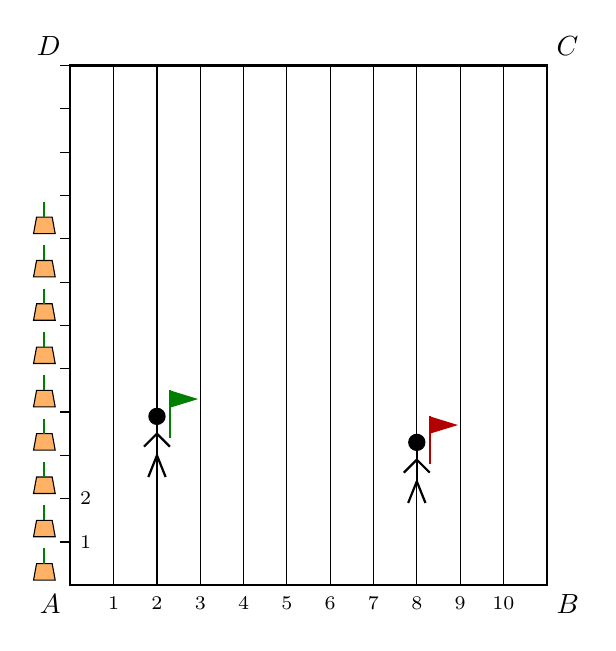
\begin{tikzpicture}[scale=0.55]
% the field: 11 m wide, drawn tall; the 10 chalk lines are 1 m apart
\draw[thick] (0,0) rectangle (11,12);
\foreach \x in {1,...,10}{\draw (\x,0)--(\x,12); \node[below,font=\scriptsize] at (\x,-0.05) {\x};}
% flower pots along AD (only the lower ones drawn), tick marks every metre
\foreach \i in {0,...,8}{%
  \draw[fill=orange!60] (-0.85,\i+0.12)--(-0.35,\i+0.12)--(-0.42,\i+0.5)--(-0.78,\i+0.5)--cycle;
  \draw[green!50!black,thick] (-0.6,\i+0.5)--(-0.6,\i+0.85);}
\foreach \i in {1,...,12}{\draw (-0.25,\i)--(0,\i);}
\node[right,font=\scriptsize] at (0,1) {1};
\node[right,font=\scriptsize] at (0,2) {2};
% the two runners with their flags (positions as in the question)
\begin{scope}[shift={(2,3)}]
 \draw[thick] (0,0)--(0,0.7); \draw[thick] (0,0)--(-0.2,-0.5); \draw[thick] (0,0)--(0.2,-0.5);
 \draw[thick] (0,0.5)--(0.3,0.2); \draw[thick] (0,0.5)--(-0.3,0.2); \fill (0,0.9) circle (0.2);
 \draw[green!50!black,thick] (0.3,0.4)--(0.3,1.5); \fill[green!50!black] (0.3,1.5)--(0.95,1.3)--(0.3,1.1)--cycle;
\end{scope}
\begin{scope}[shift={(8,2.4)}]
 \draw[thick] (0,0)--(0,0.7); \draw[thick] (0,0)--(-0.2,-0.5); \draw[thick] (0,0)--(0.2,-0.5);
 \draw[thick] (0,0.5)--(0.3,0.2); \draw[thick] (0,0.5)--(-0.3,0.2); \fill (0,0.9) circle (0.2);
 \draw[red!70!black,thick] (0.3,0.4)--(0.3,1.5); \fill[red!70!black] (0.3,1.5)--(0.95,1.3)--(0.3,1.1)--cycle;
\end{scope}
\node[below left] at (0,0) {$A$};\node[below right] at (11,0) {$B$};
\node[above right] at (11,12) {$C$};\node[above left] at (0,12) {$D$};
\end{tikzpicture}%
\figcap{Fig.\ 7.12 (redrawn, not to scale). Chalk lines numbered $1$ to $10$ from $A$ along $AB$; flower pots 1~m apart along $AD$ (only some are drawn); green flag on line 2, red flag on line 8.}
\end{center}

\textbf{Solution.}

\textbf{Step 1: length of $AD$.} 100 flower pots are placed 1~m apart along $AD$, so $AD=100$~m (this is the value the book intends).

\textbf{Step 2: set up coordinates.} Take $A$ as the origin, $AB$ along the $x$-axis and $AD$ along the $y$-axis, with 1 unit = 1~m. The chalk lines are 1~m apart and numbered from $A$, so the $n$th line is the line $x=n$. A flag on the $n$th line therefore has $x$-coordinate $n$, and its $y$-coordinate is its distance from $AB$ measured along the line.
\slip{``The 2nd line'' gives the $x$-coordinate ($x=2$), not the $y$-coordinate. The fraction of $AD$ gives the $y$-coordinate.}

\textbf{Step 3: position of each flag.}\\
Green flag: on the 2nd line, so $x=2$. Niharika runs $\frac14$ of $AD$, so $y=\frac14\times100=25$. So $G(2,25)$.\\
Red flag: on the 8th line, so $x=8$. Preet runs $\frac15$ of $AD$, so $y=\frac15\times100=20$. So $R(8,20)$.

\textbf{Step 4: distance between the flags.} By the distance formula $d=\sqrt{(x_2-x_1)^2+(y_2-y_1)^2}$ with $(x_1,y_1)=(2,25)$ and $(x_2,y_2)=(8,20)$:
\begin{align*}
\distn{GR}{2}{25}{8}{20}
\end{align*}
$\sqrt{61}\approx7.81$ and $61$ has no square factor, so it stays as $\sqrt{61}$.

\textbf{Step 5: the blue flag.} Rashmi posts it halfway between the two flags, that is at the mid-point of $GR$. By the mid-point formula $\left(\dfrac{x_1+x_2}{2},\dfrac{y_1+y_2}{2}\right)$:
\[
\left(\frac{2+8}{2},\ \frac{25+20}{2}\right)=\left(\frac{10}{2},\ \frac{45}{2}\right)=(5,\ 22.5).
\]

\textbf{Verification.} The blue flag $B_1(5,22.5)$ should be equally far from both flags. Using $d^2=(x_2-x_1)^2+(y_2-y_1)^2$:
\begin{align*}
B_1G^2&=(2-5)^2+(25-22.5)^2=(-3)^2+(2.5)^2=9+6.25=15.25\\
B_1R^2&=(8-5)^2+(20-22.5)^2=3^2+(-2.5)^2=9+6.25=15.25
\end{align*}
Each is $15.25=\dfrac{61}{4}$, so each distance is $\dfrac{\sqrt{61}}{2}$, which is half of $GR$.

\ans{The distance between the two flags is $\sqrt{61}$ m ($\approx7.81$ m). Rashmi should post the blue flag at $(5,22.5)$, that is on the 5th line, $22.5$ m from $AB$ along that line.}

%---------------------------------------------------------------
\subsection*{Exercise 7.2, Question 4}
\textbf{Question.} Find the ratio in which the line segment joining the points $(-3,10)$ and $(6,-8)$ is divided by $(-1,6)$.

\textbf{Solution.} Let $A(-3,10)$, $B(6,-8)$ and let $P(-1,6)$ divide $AB$ in the ratio $m_1:m_2$. So $(x_1,y_1)=(-3,10)$ and $(x_2,y_2)=(6,-8)$.

By the section formula, $x=\dfrac{m_1x_2+m_2x_1}{m_1+m_2}$:
\begin{align*}
-1&=\frac{m_1(6)+m_2(-3)}{m_1+m_2}=\frac{6m_1-3m_2}{m_1+m_2}\\
-(m_1+m_2)&=6m_1-3m_2\\
-m_1-m_2&=6m_1-3m_2\\
3m_2-m_2&=6m_1+m_1\\
2m_2&=7m_1\\
\frac{m_1}{m_2}&=\frac27
\end{align*}
So the ratio is $2:7$.

\textbf{Check with the $y$-coordinate.} Put $m_1=2$, $m_2=7$ in $y=\dfrac{m_1y_2+m_2y_1}{m_1+m_2}$:
\[\frac{2(-8)+7(10)}{2+7}=\frac{-16+70}{9}=\frac{54}{9}=6,\]
which is the $y$-coordinate of $P$. The ratio is correct.

\ans{The ratio is $2:7$.}

%---------------------------------------------------------------
\subsection*{Exercise 7.2, Question 5}
\textbf{Question.} Find the ratio in which the line segment joining $A(1,-5)$ and $B(-4,5)$ is divided by the $x$-axis. Also find the coordinates of the point of division.

\textbf{Solution.} Let the $x$-axis divide $AB$ at $P$ in the ratio $k:1$. A point on the $x$-axis has $y$-coordinate $0$. Here $(x_1,y_1)=(1,-5)$, $(x_2,y_2)=(-4,5)$, $m_1=k$, $m_2=1$.

By the section formula $\left(\dfrac{m_1x_2+m_2x_1}{m_1+m_2},\dfrac{m_1y_2+m_2y_1}{m_1+m_2}\right)$:
\[
P=\left(\frac{k(-4)+1(1)}{k+1},\ \frac{k(5)+1(-5)}{k+1}\right)=\left(\frac{1-4k}{k+1},\ \frac{5k-5}{k+1}\right).
\]
The $y$-coordinate of $P$ is $0$:
\[\frac{5k-5}{k+1}=0\ \Rightarrow\ 5k-5=0\ \Rightarrow\ k=1 .\]
So the ratio is $1:1$. Put $k=1$ in the $x$-coordinate:
\[x=\frac{1-4(1)}{1+1}=\frac{-3}{2}=-\frac32 .\]

\textbf{Verification.} A ratio $1:1$ means $P$ is the mid-point. By the mid-point formula,
\[
\left(\dfrac{x_1+x_2}{2},\dfrac{y_1+y_2}{2}\right)
\]
the mid-point of $AB$ is
\[
\left(\dfrac{1+(-4)}{2},\dfrac{-5+5}{2}\right)=\left(-\dfrac32,0\right),
\]
which lies on the $x$-axis.

\ans{The $x$-axis divides $AB$ in the ratio $1:1$ (at its mid-point), and the point of division is $\left(-\dfrac32,0\right)$.}

%---------------------------------------------------------------
\subsection*{Exercise 7.2, Question 6}
\textbf{Question.} If $(1,2)$, $(4,y)$, $(x,6)$ and $(3,5)$ are the vertices of a parallelogram taken in order, find $x$ and $y$.

\textbf{Solution.} Let $A(1,2)$, $B(4,y)$, $C(x,6)$, $D(3,5)$. The diagonals of a parallelogram bisect each other, so the mid-points of the diagonals $AC$ and $BD$ coincide.

By the mid-point formula $\left(\dfrac{x_1+x_2}{2},\dfrac{y_1+y_2}{2}\right)$:
\[
\begin{gathered}
\text{Mid-point of }AC=\left(\frac{1+x}{2},\frac{2+6}{2}\right)=\left(\frac{1+x}{2},4\right),\\
\text{Mid-point of }BD=\left(\frac{4+3}{2},\frac{y+5}{2}\right)=\left(\frac72,\frac{y+5}{2}\right).
\end{gathered}
\]
Equate the $x$-coordinates and the $y$-coordinates:
\[
\frac{1+x}{2}=\frac72\ \Rightarrow\ 1+x=7\ \Rightarrow\ x=6,\qquad 4=\frac{y+5}{2}\ \Rightarrow\ y+5=8\ \Rightarrow\ y=3 .
\]

\textbf{Verification.} With $A(1,2)$, $B(4,3)$, $C(6,6)$, $D(3,5)$, opposite sides should be equal. By $d^2=(x_2-x_1)^2+(y_2-y_1)^2$:
\begin{align*}
AB^2&=(4-1)^2+(3-2)^2=3^2+1^2=9+1=10\\
DC^2&=(6-3)^2+(6-5)^2=3^2+1^2=9+1=10\\
BC^2&=(6-4)^2+(6-3)^2=2^2+3^2=4+9=13\\
AD^2&=(3-1)^2+(5-2)^2=2^2+3^2=4+9=13
\end{align*}
So $AB=DC$ and $BC=AD$: opposite sides are equal.

\ans{$x=6$ and $y=3$.}

%---------------------------------------------------------------
\subsection*{Exercise 7.2, Question 7}
\textbf{Question.} Find the coordinates of a point $A$, where $AB$ is the diameter of a circle whose centre is $(2,-3)$ and $B$ is $(1,4)$.

\textbf{Solution.} The centre of a circle is the mid-point of every diameter. Let $A(x,y)$ and $B(1,4)$; the centre $(2,-3)$ is the mid-point of $AB$.

By the mid-point formula $\left(\dfrac{x_1+x_2}{2},\dfrac{y_1+y_2}{2}\right)$:
\[
\frac{x+1}{2}=2\ \Rightarrow\ x+1=4\ \Rightarrow\ x=3,\qquad \frac{y+4}{2}=-3\ \Rightarrow\ y+4=-6\ \Rightarrow\ y=-10 .
\]

\textbf{Verification.} The mid-point of $A(3,-10)$ and $B(1,4)$ is $\left(\dfrac{3+1}{2},\dfrac{-10+4}{2}\right)=\left(\dfrac42,\dfrac{-6}{2}\right)=(2,-3)$, the given centre.

\ans{$A$ is $(3,-10)$.}

%---------------------------------------------------------------
\subsection*{Exercise 7.2, Question 8}
\textbf{Question.} If $A$ and $B$ are $(-2,-2)$ and $(2,-4)$, respectively, find the coordinates of $P$ such that $AP=\dfrac37AB$ and $P$ lies on the line segment $AB$.

\textbf{Solution.} Since $P$ lies on segment $AB$, $PB=AB-AP=AB-\frac37AB=\frac47AB$.
Therefore $AP:PB=\frac37AB:\frac47AB=3:4$.

By the section formula $\left(\dfrac{m_1x_2+m_2x_1}{m_1+m_2},\dfrac{m_1y_2+m_2y_1}{m_1+m_2}\right)$ with $A(-2,-2)$, $B(2,-4)$ and $m_1:m_2=3:4$:
\begin{align*}
x&=\frac{3(2)+4(-2)}{3+4}=\frac{6-8}{7}=-\frac27\\
y&=\frac{3(-4)+4(-2)}{3+4}=\frac{-12-8}{7}=-\frac{20}{7}
\end{align*}
\slip{$AP=\frac37AB$ does not mean the ratio is $3:7$. The ratio $AP:PB$ is $3:4$, because $PB=AB-AP=\frac47AB$.}

\textbf{Verification.} By the distance formula $d=\sqrt{(x_2-x_1)^2+(y_2-y_1)^2}$:
\begin{align*}
AB&=\sqrt{(2-(-2))^2+(-4-(-2))^2}=\sqrt{4^2+(-2)^2}=\sqrt{16+4}=\sqrt{20}=2\sqrt5\\
AP&=\sqrt{\left(-\tfrac27-(-2)\right)^2+\left(-\tfrac{20}{7}-(-2)\right)^2}=\sqrt{\left(\tfrac{12}{7}\right)^2+\left(-\tfrac67\right)^2}=\sqrt{\tfrac{144}{49}+\tfrac{36}{49}}=\sqrt{\tfrac{180}{49}}=\tfrac{6\sqrt5}{7}
\end{align*}
and $\frac37AB=\frac37\times2\sqrt5=\frac{6\sqrt5}{7}=AP$.

\ans{$P\left(-\dfrac27,-\dfrac{20}{7}\right)$.}

%---------------------------------------------------------------
\subsection*{Exercise 7.2, Question 9}
\textbf{Question.} Find the coordinates of the points which divide the line segment joining $A(-2,2)$ and $B(2,8)$ into four equal parts.

\textbf{Solution.} Let $P$, $Q$, $R$ be the points that divide $AB$ into four equal parts, in order from $A$. Then $P$ divides $AB$ in the ratio $1:3$, $Q$ is the mid-point of $AB$ (ratio $2:2=1:1$), and $R$ divides $AB$ in the ratio $3:1$. Here $(x_1,y_1)=(-2,2)$ and $(x_2,y_2)=(2,8)$.

By the section formula $\left(\dfrac{m_1x_2+m_2x_1}{m_1+m_2},\dfrac{m_1y_2+m_2y_1}{m_1+m_2}\right)$:

$P$ ($m_1:m_2=1:3$): $x=\dfrac{1(2)+3(-2)}{1+3}=\dfrac{2-6}{4}=-1$, $y=\dfrac{1(8)+3(2)}{1+3}=\dfrac{8+6}{4}=\dfrac{14}{4}=\dfrac72$.

$Q$ (mid-point formula $\left(\dfrac{x_1+x_2}{2},\dfrac{y_1+y_2}{2}\right)$): $x=\dfrac{-2+2}{2}=0$, $y=\dfrac{2+8}{2}=5$.

$R$ ($m_1:m_2=3:1$): $x=\dfrac{3(2)+1(-2)}{3+1}=\dfrac{6-2}{4}=1$, $y=\dfrac{3(8)+1(2)}{3+1}=\dfrac{24+2}{4}=\dfrac{26}{4}=\dfrac{13}{2}$.

\textbf{Verification.} $Q$ should be the mid-point of $PR$: $\left(\dfrac{-1+1}{2},\dfrac{\frac72+\frac{13}{2}}{2}\right)=\left(0,\dfrac{10}{2}\right)=(0,5)=Q$.

\ans{The points are $P\left(-1,\dfrac72\right)$, $Q(0,5)$ and $R\left(1,\dfrac{13}{2}\right)$.}

%---------------------------------------------------------------
\subsection*{Exercise 7.2, Question 10}
\textbf{Question.} Find the area of a rhombus if its vertices are $(3,0)$, $(4,5)$, $(-1,4)$ and $(-2,-1)$ taken in order. [Hint: Area of a rhombus $=\frac12$ (product of its diagonals)]

\textbf{Solution.} Let $A(3,0)$, $B(4,5)$, $C(-1,4)$, $D(-2,-1)$. The diagonals are $AC$ and $BD$. By the distance formula $d=\sqrt{(x_2-x_1)^2+(y_2-y_1)^2}$:

\distnote
\begin{align*}
\dist{AC}{3}{0}{-1}{4}{4\sqrt2}\\
\dist{BD}{4}{5}{-2}{-1}{6\sqrt2}
\end{align*}
(Here $\sqrt{32}=\sqrt{16\times2}=4\sqrt2$ and $\sqrt{72}=\sqrt{36\times2}=6\sqrt2$.)

By the hint, $\text{Area}=\dfrac12\,d_1d_2$ with $d_1=4\sqrt2$ and $d_2=6\sqrt2$:
\[
\text{Area}=\frac12\times4\sqrt2\times6\sqrt2=\frac12\times(4\times6)\times(\sqrt2\times\sqrt2)=\frac12\times24\times2=24 .
\]
\slip{The area is $\frac12d_1d_2$, not $d_1d_2$. Do not forget the $\frac12$.}

\textbf{Verification that $ABCD$ is a rhombus.} All four sides should be equal:
\begin{align*}
\distn{AB}{3}{0}{4}{5}\\
\distn{BC}{4}{5}{-1}{4}\\
\distn{CD}{-1}{4}{-2}{-1}\\
\distn{DA}{-2}{-1}{3}{0}
\end{align*}
All four sides are $\sqrt{26}$, so the quadrilateral is a rhombus and the hint applies.

\ans{The area of the rhombus is $24$ square units.}


\end{document}
